\begin{comment}
\begin{figure}[h]
    \centering
    %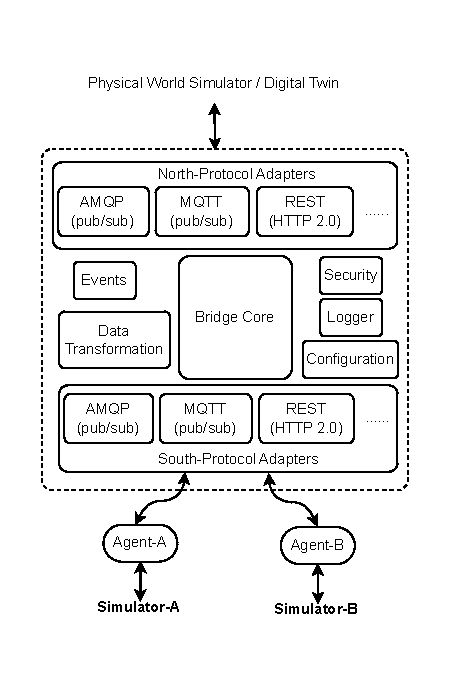
\includegraphics[width=\linewidth]{img/simulation_bridge.pdf}
    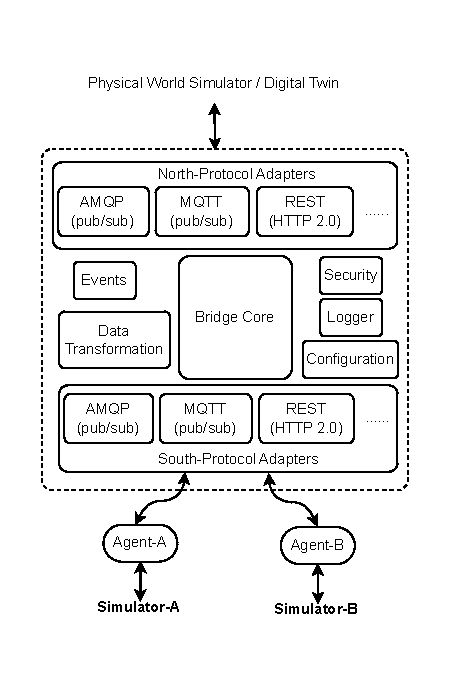
\includegraphics[width=0.7\linewidth, trim={0.1in 0.5in 0.1in 0.5in}, clip]{img/simulation_bridge.pdf}
    \caption{Architecture of the simulation bridge.}
    \label{fig:simulation_bridge_architecture}
\end{figure}   
\end{comment}

\begin{figure*}[h]
    \centering
    \subfloat[Simulation bridge architecture.]{
        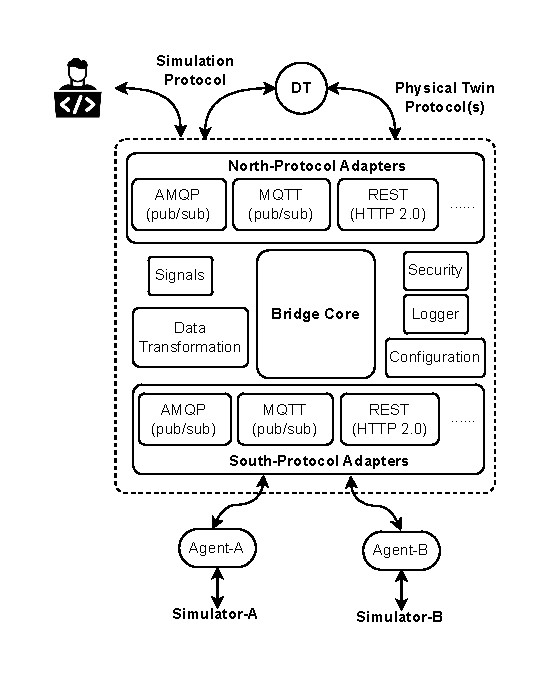
\includegraphics[width=0.35\linewidth]{img/simulation_bridge_v2.pdf}
        \label{fig:simulation_bridge_components}
    }
    \hfill
    \subfloat[Communication flow in the simulation bridge.]{
        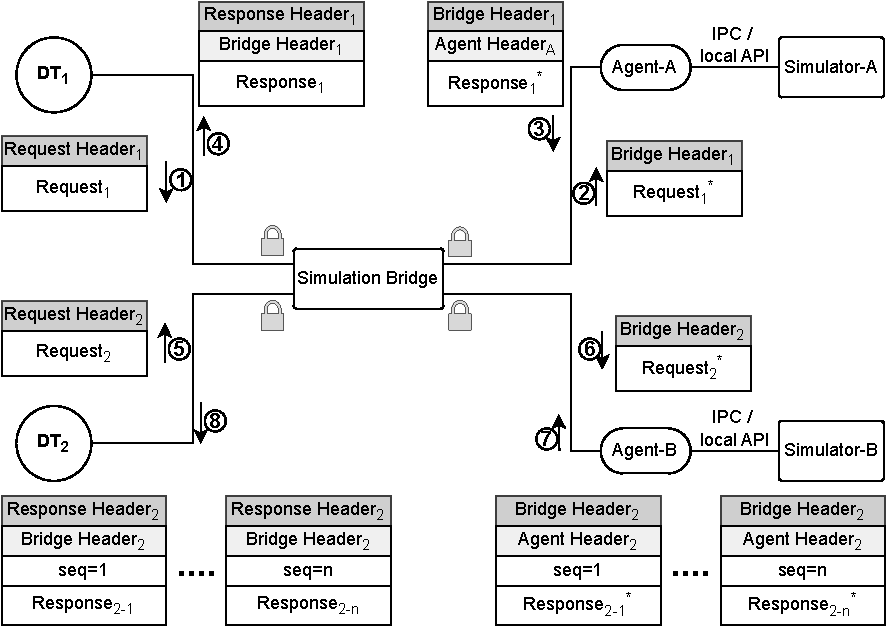
\includegraphics[width=0.56\linewidth]{img/network-setup.pdf}
        \label{fig:simulation_bridge_protocol}
    }
    \caption{Architecture of the Simulation Bridge with its main components and the associated interaction flows.}
    % \Description{Architecture of the Simulation Bridge: (a) modular components supporting DT interaction and developer-driven PT simulation, and (b) communication flow between DTs, the bridge, and simulators for simulation control and integration.}
    \label{fig:simulation_bridge_architecture}
    \vspace{-0.5cm}
\end{figure*}


\section{Simulation Bridge Architecture}
\label{sec:sim_bridge_arch}

The DT-SB coordinates heterogeneous and distributed simulations, providing a unified interface for DTs to access diverse simulation resources regardless of modeling and technological differences.
The bridge serves as a middleware which routes simulation execution requests, aggregates results, and returns them to clients. This enables seamless integration, reusability, and interoperability across simulation platforms.
% The DT-SB is designed to manage and execute heterogeneous and distributed simulations, serving as a middleware layer that facilitates interaction between DTs and a federation of simulators.
% Its primary objective is to offer a unified interface through which clients, namely DTs, can interact with a diverse set of simulation resources. 
% These simulators vary widely in their engineering paradigms, modeling approaches, and underlying implementation technologies.
% To address this diversity, the DT-SB operates as an intelligent coordination layer, responsible for routing client requests to the appropriate simulators, aggregating the resulting data, and delivering it back to the requesting clients.
% This abstraction enables seamless integration and orchestration of simulation services across heterogeneous platforms, fostering reusability, scalability, and interoperability within DT-driven ecosystems.

Figure~\ref{fig:simulation_bridge_components} illustrates the modular architecture of the DT-SB. 
At the heart of this architecture is the DT-SB, each simulator is integrated through a dedicated simulation agent (SA) module.
SAs implement a standardized uniform API layer based on a simple application protocol. 
These agents are deployed within their respective simulation environments and are responsible for interpreting incoming messages, controlling the execution of simulation tasks, and aggregating the results for transmission back to the DT-SB.
% This agent-based design ensures system-wide interoperability and enables seamless coordination across a diverse set of simulation environments.
%
Each module of the DT-SB is designed to fulfill a specific function within the operational workflow:
%. A concise description of the principal components is provided below.

\noindent\textbf{Bridge Core:}  
Serves as the central control unit of the DT-SB. It coordinates interactions among internal modules, monitors communication flows, and orchestrates message routing between external clients (e.g., DTs, PTs, simulators) and the distributed simulation environment.

\noindent\textbf{Protocol Adapters (PAs):}  
facilitate protocol translation and connection management between the DT-SB and external entities. They operate on both the north-bound interface (connecting to DTs and PTs) and the south-bound interface (connecting to SAs). PAs are implemented using a plugin architecture, allowing the system to be extended in a modular fashion.

\noindent\textbf{Event Manager:}  
DT-SB adopts an event-driven architecture, wherein all relevant actions within a PA (e.g., message transmission, reception, connection management) are internally represented as events. When a request or response is received by a PA, it is transformed into an internal event and processed by the Bridge Core.

\noindent\textbf{Data Transformation Manager:} 
is responsible for converting data formats for both incoming and outgoing communication. Transformation parameters are dynamically configurable to optimize message structures for transmission efficiency. The module supports configurable message granularity, enabling the system to manage both atomic events and composite result packets based on application requirements.

\noindent\textbf{Configuration Manager:}  
handles the validation and loading of system parameters, including supported protocols, access credentials, and routing rules. A centralized configuration approach facilitates maintainability and control. The configuration also specifies a whitelist of authorized DTs and SAs.
%, where DTs are identified via client identifiers and SAs by the \emph{simulation types} they support.
%Simulation types abstract the behavior of the DT by combining models with associated simulation methods. While DTs may specify models for simulation, local configurations may influence execution behavior even with a given model-simulator pairing.

\noindent\textbf{Logger:}  
records internal operations, exceptions, and diagnostic messages. It also provides performance metrics and operational insights essential for monitoring and debugging the DT-SB.

\noindent\textbf{Security Manager:}  
oversees the generation and loading of TLS certificates, ensuring secure communication channels. It is also responsible for detecting and mitigating malicious activity, such as message flooding, that could lead to denial-of-service conditions targeting simulators.

\subsection{Simulator Protocol}
\label{subsec:sim-protocol}

As DTs, DT-SB, and SAs operate in a distributed system, a dedicated \emph{Simulation Protocol} (SP) serves as the unifying layer for managing simulation requests and responses. The protocol defines standard headers for request routing and result interpretation. PAs integrated into DT-SB provide their own delivery semantics; however, best-effort delivery is universally supported, making it a practical foundation for interactions with SAs. Simulators can advertise the \emph{Simulation Type (ST)} they support (an abstraction that defines expected behaviors and model-method combinations). DTs may then select one of the available STs, while the DT-SB is responsible for routing and translating the corresponding simulation requests to the appropriate SAs that provide the selected ST.

The DT-SB performs two key operations to mediate this interaction:
(i) \emph{data transformation} of simulation requests and responses to ensure syntactic and semantic consistency, and
(ii) \emph{protocol header replacement} to enforce proper message routing between DTs and the selected SAs.
Figure~\ref{fig:simulation_bridge_protocol} depicts the message exchange flow for both batch and streaming simulation modes.
Secure variants of PAs are also illustrated. 
Numbered arrows indicate the sequence of message exchanges.


\paragraph{Batch Request}
In this scenario, $DT_1$ issues a simulation request targeting a Simulation Type supported by \emph{Simulator-A} (message $m_1$, denoted as \textcircled{1} in Figure~\ref{fig:simulation_bridge_protocol}). The request includes the model name, associated model parameters, simulator input values, and the specification of required outputs.
Upon receiving the request, the DT-SB replaces the original request header with a bridge-specific header. This header replacement ensures the necessary abstraction and transparency between DTs and SAs, decoupling clients from simulator-specific implementations. The DT-SB also performs a data transformation step to normalize the request format before forwarding it to \emph{Agent-A} (message $m_2$).
Agent-A then transmits the transformed request to \emph{Simulator-A}, which executes the simulation. The resulting outputs are sent back to the DT-SB via Agent-A (message $m_3$). Agent-A attaches a custom response header containing metadata relevant to the simulation run.
Upon receiving the response, the DT-SB applies a reverse data transformation tailored to the expectations of $DT_1$, replaces the agent-specific header with a standardized response header derived from the original request metadata, and delivers the final message to $DT_1$ (message $m_4$).
All headers in the message exchange carry metadata useful for distributed tracing, debugging, and performance analysis, thereby supporting observability and diagnostics across the system.


\paragraph{Streaming Request}
In this scenario, $DT_2$ initiates a simulation request targeting \emph{Simulator-B} (message $m_5$, denoted as \textcircled{5} in Figure~\ref{fig:simulation_bridge_protocol}). As with batch requests, the DT-SB intercepts the request, applies the necessary data transformation, and replaces the header with a bridge-specific version before forwarding the request to \emph{Agent-B} (message $m_6$). Agent-B then relays the request to \emph{Simulator-B}, which begins executing the streaming simulation.
Unlike batch simulations, streaming simulations generate a sequence of response messages over time. To ensure that responses are interpreted in the correct order, Agent-B attaches a sequence number to each outgoing message. This sequence number enables both DT-SB and $DT_2$ to preserve the temporal order of the response stream.
Agent-B forwards the ordered sequence of responses to the DT-SB (denoted as multiple instances of message $m_7$), which in turn applies reverse data transformation and forwards the processed responses to $DT_2$ (messages $m_8$).
In Figure~\ref{fig:simulation_bridge_protocol}, these streaming responses have $seq$ number field which is used by $DT_2$ to arrange the streaming responses in the correct order.

\paragraph{PT Simulation}

For the simulation of PTs, the DT-SB is used by two distinct entities. On one side, the developer interacts with the bridge through the simulation protocol and the north-protocol adapters to configure and launch simulations, define the mapping of simulated entities, and specify how these entities are exposed to the digital world via specific protocols, for example by mapping a simulation entity to MQTT. On the other side, the DT receives data from the simulated PTs through the configured protocols as if it were coming from the actual physical objects that will feed the DT in real deployments. Communication between the DT and the DT-SB is bidirectional: the DT not only receives telemetry data from the simulated PTs but can also send actions. These actions are translated by the bridge into commands for the simulation, modifying the behavior of the simulated PTs via interactions managed through the protocols and simulation agents enabled by the south-protocol adapters.


%\hl{hard to match the stuff below with figure}

\begin{comment}
In Figure~\ref{fig:simulation_bridge_protocol}, these responses are labeled as $Response_{2\text{-}k}$, where the first subscript ($2$) denotes the originating DT (i.e., $DT_2$), and the second subscript ($k$) denotes the position in the response sequence. Both DT-SB and $DT_2$ rely on the sequence number embedded in each response to ensure correct processing and ordered delivery of simulation outputs.
\end{comment}


\subsection{Routing Messages}

%Simulators often expose non-standard interfaces, which vary significantly in terms of programming abstractions and platform dependencies. Some simulators offer APIs in high-level programming languages, while others provide operating system-specific bindings. For instance, \emph{Matlab} exposes a Python API, whereas \emph{Simul8} provides a COM-based interface that is limited to the Windows operating system. Additionally, several simulators support traditional inter-process communication (IPC) mechanisms such as files, named pipes, network sockets, and shared memory. Among these, shared memory enables the most tightly coupled integration between SAs and the simulator, offering low-latency, high-throughput communication. In contrast, network socket-based interfaces allow greater deployment flexibility by enabling the SA and its associated simulator to reside on different nodes within a distributed system.

A critical responsibility of the DT-SB is to map incoming simulation responses to their corresponding requests. This mapping is maintained using a dynamic routing table, with representative entries illustrated in Table~\ref{tab:index-table}. 

\begin{table}[h]
    \centering
    \caption{DT-SB's routing table.}
    \label{tab:index-table}
    \renewcommand{\arraystretch}{1.5}  % Adjust this factor to achieve 12pt spacing
    \begin{tabular}{p{0.5in}llp{0.5in}lp{0.5in}}
    \hline
    \textbf{$PA_N$} & \textbf{$PA_S$} & \textbf{DT} & \textbf{Sim. Type} & \textbf{Request-id} & \textbf{Timeout}\\
    \hline
    MQTT & AMQP & $DT_1$ & Octave & $hash\#1$ & 60s\\
    AMQP & MQTT & $DT_1$ & Matlab & $hash\#2$ & 60s\\
    REST & AMQP & $DT_2$ & Simul8 & $hash\#3$ & 120s\\
    \hline
    \end{tabular}
\end{table}

% \begin{table}[h]
%     \centering
%     \caption{Routing table used by DT-SB for internal message routing.}
%     \label{tab:index-table}
%     \renewcommand{\arraystretch}{1.5}  % Adjust this factor to achieve 12pt spacing
%     \begin{tabular}{p{0.5in}llp{0.5in}lp{0.5in}}
%     \hline
%     \textbf{$PA_N$} & \textbf{$PA_S$} & \textbf{DT} & \textbf{Simulator Type} & \textbf{Request-id} & \textbf{Timeout (seconds)}\\
%     \hline
%     MQTT & AMQP & $DT_1$ & Octave & $hash\#1$ & 60\\
%     AMQP & MQTT & $DT_1$ & Matlab & $hash\#2$ & 60\\
%     REST (HTTP/2.0) & AMQP & $DT_2$ & Simul8 & $hash\#3$ & 120\\
%     \hline
%     \end{tabular}
% \end{table}

The column $PA_N$ denotes the PA selected by the DT, while $PA_S$ represents the PA associated with the Simulator Agent. In scenarios where the DT-SB supports only a single protocol on either the north-bound ($PA_N$) or south-bound ($PA_S$) interface, the corresponding column can be omitted to simplify the routing logic.
The \emph{Simulator Type} column identifies the class of simulations handled by a given SA. Each simulation request is uniquely identified by a \texttt{RequestID}, which may be generated using hash-based algorithms to ensure uniqueness and unpredictability. A timeout field is also included to define the expiration threshold for requests; expired entries are purged to maintain routing table efficiency. When a simulation response arrives, the tuple $\langle PA_S, ST, \texttt{RequestID} \rangle$ is extracted and matched against existing routing table entries. The identified row provides the target DT and the associated $PA_N$, allowing the DT-SB to correctly route the response back to the originating DT. This mechanism ensures correct correlation of simulation data even in asynchronous or distributed execution contexts.




\begin{comment}
\begin{figure}[h]
    \centering
    
\includegraphics[height=4cm]{img/event_based_sm.pdf}
    \caption{Event-Based Architecture\textcolor{blue}{replace with a table}}
    \label{fig:event_based_sm}
\end{figure}

The \textit{sim-bridge} is a sophisticated software platform involving advanced engineering challenges, designed to execute heterogeneous distributed simulations. 
Its primary goal is to enable an external client to interact in a simple and transparent way with a network of distributed simulators, which may differ significantly in terms of nature, technology, and location.

The role of the sim-bridge project is therefore to act as an intelligent intermediary between the client and the various simulators, handling the routing of incoming requests to the appropriate simulator, collecting the results, and delivering them back to the client in a secure and efficient manner. In this context, \textit{sim-bridge} not only ensures uniform access to distributed simulation resources, but also abstracts the underlying complexities arising from their heterogeneity.

\begin{figure}[h]
    \centering
    
\includegraphics[height=4cm]{img/simulation_bridge_overview.pdf}
    \caption{\textit{sim-bridge} Overview}
    \label{fig:simulation_bridge_overview}
\end{figure}    

To enable this functionality, a central component, the \textit{sim-bridge}, has been designed to handle the routing of requests across multiple communication protocols and to manage the distributed nature of the simulators. In order to be integrated into the system, each simulator requires a dedicated agent that acts as an internal interpreter between the simulator's proprietary APIs and the \textit{sim-bridge} (Figure~\ref{fig:agent_role}).

To address the challenges posed by the diversity of proprietary languages, complex connectors, and custom APIs, together with the absence of a universally accepted standard protocol, a dedicated agent has been developed for each simulator. 

Each simulator is thus paired with its own agent, which implements a common interface shared among all agents. This standardized interface defines the APIs and communication methods used to interact with the various simulators, ensuring both consistency and interoperability within the system.

\begin{figure}[h]
    \centering
    
\includegraphics[height=5cm]{img/agent_role.pdf}
    \caption{Agent Role}
    \label{fig:agent_role}
\end{figure}

Communication between clients and the \textit{Simulation Bridge} is flexible and location-independent. As depicted in Figure~\ref{fig:position_sm}, this communication can occur either directly at the client’s edge or within the system core, depending on each Digital Twin or Mock Physical Twin’s capability to support specific communication protocols.

\begin{figure}[h]
    \centering
    
\includegraphics[height=6cm]{img/position_sm.pdf}
    \caption{Communication between clients and \textit{sim-bridge}}
    \label{fig:position_sm}
\end{figure}    

\begin{figure}[h]
    \centering
    
\includegraphics[height=6cm]{img/project.pdf}
    \caption{Structure of the Simulation Bridge}
    \label{fig:structure}
\end{figure}

Figure~\ref{fig:structure} illustrates the modular architecture of the \textit{sim-bridge} and its main software components. Each module is designed to perform a specific function within the overall operational workflow.

\textbf{Protocol Adapter}

The \textit{Protocol Adapter} module is responsible for translating and managing connections between the \textit{sim-bridge} and various communication protocols. In the initial version, the \textit{sim-bridge} supports RabbitMQ, MQTT, and HTTP. This component is designed with a plugin architecture, allowing easy extension to support new protocols, thus ensuring flexibility and adaptability to future requirements.

\textbf{Data Transformation Manager}

The \textit{Data Transformation Manager} handles the transformation of incoming and outgoing data, adapting it to the formats required by simulators or production systems. This module allows configurable management of message granularity, supporting both single events and complete result packets, depending on the needs of the application context. The configurability of the transformation level enables dynamic selection of the data format and structure to be transmitted.

\textbf{Config Manager}

The \textit{sim-bridge} is fully configurable via YAML files. The \textit{Config Manager} is responsible for reading, validating, and loading this configuration file, which defines the entities involved, the protocols to be used, and the rules for message routing. This approach promotes centralized and transparent configuration management, facilitating system maintenance and scalability.

\textbf{Logger}

The system integrates a customized logger that records all internal operations and handles potential errors. The logger configuration is also managed through the YAML file, allowing adjustment of the log detail level according to different operational needs (e.g., INFO, DEBUG, WARNING, ERROR, CRITICAL).

\textbf{Certs Manager}

The \textit{Certs Manager} module is responsible for generating, validating, and managing TLS security certificates, such as certfiles and keyfiles. If these certificates are missing or invalid, the manager automatically generates and stores them in the predefined folder, thus ensuring secure communications.

\textbf{\textit{sim-bridge} Core}

The \textit{Core} represents the logical heart of the system. It coordinates the internal components, monitors real-time communications, and manages message routing between external clients and distributed simulators.

\textbf{Signal Manager}

The \textit{sim-bridge} is based on an event-driven architecture, where each protocol has both an input and an output channel, each linked to internal events. When a message arrives on a protocol, it is converted into an event and handled by the core. Similarly, results follow the same process. The \textit{Signal Manager} reads the event configuration from the file \texttt{adapters\_signal.json} and automatically associates callback functions to the corresponding events, ensuring efficient event management.
Figure~\ref{fig:event_based_sm} illustrates how each protocol adapter is connected to specific events and how the core component manages these events.

\begin{figure}[h]
    \centering
    
\includegraphics[height=4cm]{img/event_based_sm.pdf}
    \caption{Event-Based Architecture}
    \label{fig:event_based_sm}
\end{figure}


\textbf{\textit{sim-bridge} Infrastructure}

The \textit{sim-bridge} uses an internal communication infrastructure based on RabbitMQ, which is necessary for secure and structured communication with the simulator agents. The connection between the \textit{sim-bridge} and the agents is stable and exclusively maintained via RabbitMQ.

\textbf{Simulator’s Agent}

The inherent challenges associated with various proprietary languages of simulators and the absence of standardized communication protocols are mitigated through an systematic agent-based approach. Each simulator is coupled with a specialized agent that conforms to a standardized interface specification. This architectural decision establishes a uniform API layer and communication methodology for simulator interactions, thereby ensuring system-wide interoperability and maintaining consistency across the distributed simulation environment.

The integration of individual simulators into this framework is accomplished through dedicated agent modules that function as interface adapters between proprietary simulator APIs and the centralized sim-bridge architecture, as depicted in Fig. 1.

The \textit{Simulator’s Agent} is a software component developed specifically for each integrated simulator. Its purpose is to act as an intermediary between the \textit{sim-bridge} and the simulator’s proprietary APIs. Each agent implements a common, standardized interface shared by all agents, allowing the \textit{sim-bridge} to interact uniformly with heterogeneous simulators. The agent must be integrated within the simulation software itself and manages message interpretation, simulation activation, and result collection to be forwarded to the \textit{sim-bridge}.

\end{comment}


